\documentclass[a4paper, 12pt]{article}%тип документа

%отступы
\usepackage[left=2cm,right=2cm,top=2cm,bottom=3cm,bindingoffset=0cm]{geometry}

%Русский язык
\usepackage[T2A]{fontenc} %кодировка
\usepackage[utf8]{inputenc} %кодировка исходного кода
\usepackage[english,russian]{babel} %локализация и переносы

%Вставка картинок
\usepackage{wrapfig}
\usepackage{graphicx}
\graphicspath{{pictures/}}
\DeclareGraphicsExtensions{.pdf,.png,.jpg}

%Графики
\usepackage{pgfplots}
\pgfplotsset{compat=1.9}

%Математика
\usepackage{amsmath, amsfonts, amssymb, amsthm, mathtools}

%Заголовок
\author{Валеев Рауф Раушанович \\
группа 8}
\title{\textbf{Работа 2.1.1 \\ 
Измерение удельной теплоемкости воздуха при постоянном давлении}}

\begin{document}
\maketitle

\section*{Цель работы}
\begin{enumerate}
\item измерение повышения температуры воздуха в результате подвода тепла при стационаром течении через стеклянную трубу;
\item Вычисление при постоянном давлении темплоемкости воздуха.
\end{enumerate}
\section*{Введение}
\subsection*{Теоретическая справка}
Измерение теплоёмкости тел обычно производится в калориметрах, т.е. в сосудах, обеспечивающих теплоизоляцию исследуемого тела от внешней среды. При этом регистрируется изменение его температуры $\delta T$ в зависимости от количества тепла $\delta Q$, полученного телом от некоторого нагревательного элемента внутри калориметра. Теплоёмкость тела в некотором процессе определяется как их отношение:
\begin{equation}
\begin{aligned}
C = \dfrac{\delta Q}{\delta T} 
\end{aligned}
\end{equation}
Надёжность измерения определяется, в основном, качеством калориметра. Необходимо, чтобы количество тепла, затрачиваемое на нагревание исследуемого тела, существенно превосходило тепло, расходуемое на нагревание самого калориметра, а также на потери тепла из установки. При измерении теплоёмкости газов эти требования выполнить довольно трудно - масса газа в калориметре и, следовательно, количество тепла, идущее на его нагревание, как правило, малы. Для увеличения количества нагреваемого газа при неизменных размерах установки в нашей работе исследуемый газ (воздух) продувается через калориметр, внутри которого установлен нагреватель. При этом измеряются мощность нагревателя, масса воздуха, протекающего в единицу времени (расход), и приращение его температуры.
\newpage
\begin{wrapfigure}{r}{0.6\textwidth}
  \begin{center}
    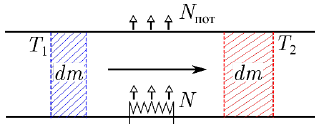
\includegraphics[width = 0.6\textwidth]{211_2.png}
  \end{center}
  \textbf{\caption{Нагрев газа при течении по трубе}}
\end{wrapfigure}
Рассмотрим газ, протекающий стационарно слева направо через трубу постоянного сечения, в кото-рой установлен нагревательный элемент (см.рис.1). Пусть за некоторое время $dt$ через калориметр прошла малая порция газа массой $dm = q dt$ , где $q$ [кг/с] - массовый расход газа в трубе. Если мощность нагрева равна $N$, мощность тепловых потерь на обмен с окружающей средой $N_{\text{пот}}$, то порция получила тепло $\delta Q =(N - N_{\text{пот}})dt$. С другой стороны, по определению теплоёмкости
(1): $\delta Q =c dm \Delta T$ , где $\Delta T = T_2 - T_1$ - приращение температуры газа, и $c$ — удельная (на единицу массы) теплоёмкость газа в рассматриваемом процессе. При малых расходах газа и достаточно большом диаметре трубы перепад давления на её концах мал, поэтому можно принять, что $P_1 \approx P_2 = P_0$, где $P_0$ - атмосферное давление. Следовательно, в условиях опыта измеряется удельная теплоёмкость при постоянном давлении $c_P$. Таким образом, получаем
\begin{equation}
\begin{aligned}
C_p = \dfrac{N - N_{\text{пот}}}{q \Delta T} 
\end{aligned}
\end{equation}
\subsection*{Экспериментальная установка}
Схема установки изображена на рис. 1. Воздух, нагнетаемый компрессором, прокачивается через калориметр. Калориметр представляет собой стеклянную цилиндрическую трубку с двойными стенками, запаянными с торцов. На внутреннюю поверхность стенок трубки нанесено серебряное покрытие для минимизации потерь тепла за счет излучения. Воздух из пространства между стенками калориметра откачан до высокого вакуума ($10^{-5}$ торр) для минимизации потерь тепла, обусловленных теплопроводностью.
\begin{center}
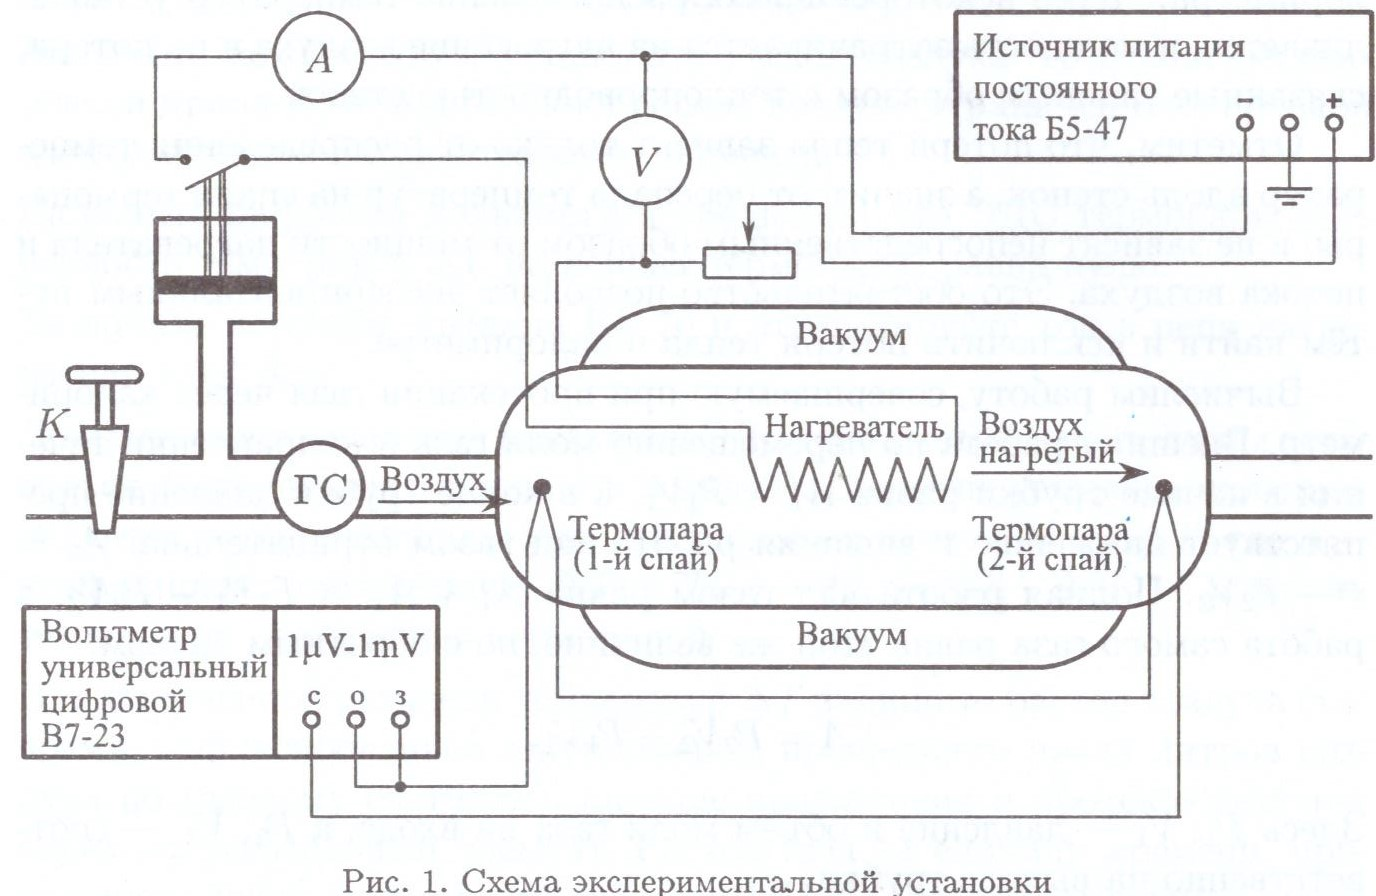
\includegraphics[width = 0.8\textwidth]{211_1.jpg}
\end{center}
Нагреватель в виде намотанной на пенопласт нихромовой проволоки раcположен внутри калориметра непосредственно в воздушном потоке. Нагрев проволоки производится от регулируемого источника постоянного тока (ИП). Напряжение $U$ на нагревателе и ток $I$ через него регистрируются цифровыми мультиметрами. Таким образом, мощность нагрева равна
\begin{equation}
\begin{aligned}
N = UI 
\end{aligned}
\end{equation}
Для измерения разности температур $\Delta T$ служит медно-константановая термопара. Один спай термопары расположен в струе воздуха, входящего в калориметр, и находится при комнатной температуре, а второй - в струе выходящего нагретого воздуха. Константановая проволока термопары расположена внутри калориметра, а медные проводники подключены к цифровому вольтметру. Возникающая в термопаре ЭДС $\varepsilon$ пропорциональна разности температур $\Delta T$ спаев:
\begin{equation}
\begin{aligned}
\varepsilon = \beta \Delta T
\end{aligned}
\end{equation}
где $\beta = 40,7 \dfrac{\text{мкВ}}{ ^{\circ} C}$ - чувствительность медно-константановой термопары в рабочем диапазоне температур (20-30 $ ^{\circ} C$). ЭДС регистрируется с помощью микровольтметра.

Объём воздуха, прошедшего через калориметр, измеряется газовым счётчиком ГС. Для регулировки расхода служит кран К. Время $\Delta t$ прохождения некоторого объема $\Delta V$ воздуха измеряется секундомером. Объёмный расход равен $\Delta V / \Delta t$, массовый расход может быть найден как
\begin{equation}
\begin{aligned}
q = \rho_0 \dfrac{\Delta V}{\Delta t} 
\end{aligned}
\end{equation}
где $\rho_0$ - плотность воздуха при комнатной температуре, которая в свою очередь может быть получена из уравнения Менделеева–Клапейрона: $\rho_0 = \dfrac{\mu P_0}{RT_0}$, где $P_0$ - атмосферное давление, $T_0$ - комнатная температура (в Кельвинах), $\mu$ = 29,0 г/моль - средняя молярная масса (сухого) воздуха.

Учитывая особенности устройства калориметра, следует ожидать, что мощность нагревателя расходуется не только на нагрев массы прокачиваемого воздуха, но и частично теряется за счет нагрева внутренних стенок термостата и рассеяния тепла через торцы термостата. Можно предположить, что при небольшом нагреве ($\Delta T << T_0$) мощность потерь тепла $N_{\text{пот}}$ прямо пропорциональна разности температур:
\begin{equation}
\begin{aligned}
N_{\text{пот}} = \alpha \Delta T
\end{aligned}
\end{equation}
где $\alpha$ — некоторая константа. При этом условии основное соотношение (2) принимает вид
\begin{equation}
\begin{aligned}
N = (c_p q+ \alpha) \Delta T
\end{aligned}
\end{equation}
Следовательно, при фиксированном расходе воздуха ($q = const$) подводимая мощность и разность температур связаны прямой пропорциональностью ($\Delta T (N)$ — линейная функция).
\section*{Ход работы}
\subsection*{Подготовка к эксперименту}
\begin{enumerate}
\item [\textbf{1.}] подготавливаем к работе газовый счетчик: проверяем, заполнен ли он водой, устанавливаем счетчик по уровню.
\item [\textbf{2.}] Начинать измерения следует при условии, что калориметр охлажден до комнатной температуры. Для охлаждения включаем компрессор и открывая кран К, устанавливаем максимально возможный расход воздуха. \textbf{Источник постоянного тока при этом выключен!}
Для проверки корректности работы газового счетчика стоит убедиться, что при постоянном расходе его стрелка вращается равномерно.
\item [\textbf{3.}] Включаем вольтметр, предназначенный для измерения ЭДС термопары. Если показания вольтметра отличны от нуля, продуваем калориметр воздухом до полного охлаждения калориметра (т.е. до установления нуля на цифровом дисплее вольтметра).
\item [\textbf{4.}]Запишем значения температуры и давления в комнате, необходимые для расчета расхода прокачиваемого воздуха. По психрометру определяем значение влажности воздуха в комнате.
\begin{center}
    \begin{tabular}{|c|c|c|}
\hline
               & Значение & $\sigma$ \\ \hline
$p$, Па        & 98340    & 1        \\ \hline
$T, ^{\circ}C$ & 25,2     & 0,1      \\ \hline
$\varphi$         & 71\%     & 1\%      \\ \hline
\end{tabular}
  \end{center}
\item [\textbf{5.}] С помощью газового счетчика и секундомера измерьте максимальный расход воздуха $\Delta V/ \Delta t$ (в л/с). Измерения проведите несколько раз и определите среднее значение расхода. Вычислите соответствующий массовый расход воздуха $q_{max} \approx 0,095$ г/с, пользуясь формулой (5).
\begin{center}
\begin{tabular}{|c|c|c|}
\hline
$\rho$, г/л & $\sigma_{\rho}$, г/л & $C_{p \text{ } theor}$, $\dfrac{\text{Дж}}{\text{г}\cdot K}$ \\\hline
1,1502      & 0,0005               & 1                                           \\ \hline
\end{tabular}

\begin{tabular}{|c|c|c|c|c|c|}
\hline
\multicolumn{6}{|c|}{1} \\
\hline
$\Delta V$, л & $\sigma_V$, л & $\Delta t, c$ & $\sigma_t$, c & $q_{max(1)}$, г/с & $\sigma_q$, г/с \\ \hline
5             & 0,1           & 60,6          & 0,5           & 0,095    & 0,002           \\ \hline
5             & 0,1           & 61,2          & 0,5           & 0,094    & 0,002           \\ \hline
5             & 0,1           & 60,8          & 0,5           & 0,095    & 0,002           \\ \hline
\end{tabular}

\begin{tabular}{|c|c|c|c|c|c|}
\hline
\multicolumn{6}{|c|}{2} \\ \hline
$\Delta V$, л & $\sigma_V$, л & $\Delta t, c$ & $\sigma_t$, c & $q_{max(1)}$, г/с & $\sigma_q$, г/с \\ \hline
2 & 0,1 & 70,7 & 0,5 & 0,033 & 0,002 \\ \hline
2 & 0,1 & 68,1 & 0,5 & 0,034 & 0,002 \\ \hline
3 & 0,1 & 103,8 & 0,5 & 0,033 & 0,002 \\ \hline
\end{tabular}

\begin{tabular}{|c|c|c|c|c|c|}
\hline
\multicolumn{6}{|c|}{3} \\ \hline
$\Delta V$, л & $\sigma_V$, л & $\Delta t, c$ & $\sigma_t$, c & $q_{max(1)}$, г/с & $\sigma_q$, г/с \\ \hline
1 & 0,1 & 60,6 & 0,5 & 0,019 & 0,002 \\ \hline
1 & 0,1 & 61,7 & 0,5 & 0,019 & 0,002 \\ \hline
1 & 0,1 & 60,3 & 0,5 & 0,019 & 0,002 \\ \hline
\end{tabular}
\end{center}
\item [\textbf{6.}] Оцениваем величину тока нагревателя $I_0$, требуемого для нагрева воздуха на $\Delta T = 1 ^{\circ}C$. Для этого определяем теоретическое значение удельной теплоёмкости воздуха при постоянном давлении $c_{p \text{ } theor}$ [Дж/г$\cdot$К], считая воздух смесью двухатомных идеальных газов; оцениваем минимальную мощность $N_0 \approx (0,095 \pm 0,003)$ Вт ($N \geq c_p q \Delta T$), необходимую для нагрева газа при максимальном расходе $q_{max}$ на $\Delta T_0 = 1^{\circ}C$; учитывая, что сопротивление проволоки нагревателя составляет приблизительно $R_H \approx 35$ Ом и в процессе опыта практически не меняется, определияем искомое значение тока $$I_0 = \sqrt{\dfrac{N_0}{R_H}} \approx (52 \pm 2) \text{ } mA$$  
\end{enumerate}
\subsection*{Проведение измерений}
\begin{enumerate}
\item [\textbf{7.}]Проведите измерение зависимости разности температур от мощности нагрева $\Delta T (N)$ при максимальном расходе воздуха $q_1 = q_{max}$. Рекомендуется измерить 4-5 точек в диапазоне температур $\Delta T$ от $\approx 2^{\circ}C$ до $\approx 10^{\circ}C$.
\begin{enumerate}
\item [\textbf{7.1}] Чтобы начать нагрев, включаем источник питания (ИП) нагревателя и устанавливаем на нём такое напряжение, чтобы ток через нить нагревателя составлял $I_1 \sim (2 \div 2,5)I_0$ (см. п. 6). Записываем значения тока $I$ и напряжения $U$ в цепи. Рассчитайте мощность $N$ нагрева, а также сопротивление нити нагревателя $R_{\text{н}}$.
\item [\textbf{7.2}] После включения нагрева (или после изменения его мощности) дожидаемся установления стационарного состояния системы. Первоначальный прогрев калориметра происходит достаточно долго ($\sim$ 10 минут). Значения ЭДС $\varepsilon$ вольтметра, подключенного к термопаре, должны оставаться постоянными (в пределах точности прибора) в течение 1-2 минут.
\item [\textbf{7.3}] По величине $\varepsilon$ определите значение $\Delta T$ (см. (4)). Учитывая, что $\Delta T \varpropto N \varpropto I^2$, определяем значения токов накала, необходимые для того, чтобы равномерно повышать температуру нагрева $\Delta T$ до требуемого значения. Проводим измерения согласно пп. 7.1.-7.2, последовательно увеличивая ток нагрева до расчётных значений.
\end{enumerate}
\item [\textbf{8.}] Повторяем измерения по п. 7 по крайней мере ещё для одного значения расхода воздуха.
\begin{center}
\begin{tabular}{|c|c|c|c|c|c|}
\hline
\multicolumn{6}{|c|}{$q_1 = (0,095 \pm0,002)$, г/c} \\ \hline
$I$, мА & 88,21 & 98,69 & 128,38 & 150,3 & 174,03 \\ \hline
$\sigma_I$, мА & 0,01 & 0,01 & 0,01 & 0,01 & 0,01 \\ \hline
$U$, В & 3,081 & 3,448 & 4,488 & 5,257 & 6,09 \\ \hline
$\sigma_U$, В & 0,001 & 0,001 & 0,001 & 0,001 & 0,001 \\ \hline
$\Delta U_{thermopara}$, мкВ & 116 & 142 & 217 & 287 & 382 \\ \hline
$\sigma_{\Delta U_{thermopara}}$, мкВ & 1 & 1 & 1 & 1 & 1 \\ \hline
$R$, Ом & 34,93 & 34,94 & 34,96 & 34,98 & 34,99 \\ \hline
$\sigma_R$, Ом & 0,01 & 0,01 & 0,01 & 0,01 & 0,01 \\ \hline
$N$, Вт & 0,2717 & 0,3403 & 0,5761 & 0,7901 & 1,0598 \\ \hline
$\sigma_N$, Вт & 0,0015 & 0,0015 & 0,0015 & 0,0015 & 0,0015 \\ \hline
$\Delta T, K$ & 2,85 & 3,49 & 5,33 & 7,05 & 9,39 \\ \hline
$\sigma_{Delta_T}, K$ & 0,02 & 0,02 & 0,02 & 0,02 & 0,02 \\ \hline
\end{tabular}

\begin{tabular}{|c|c|c|c|c|c|}
\hline
\multicolumn{6}{|c|}{$q_2 = (0,033 \pm0,001)$, г/c} \\ \hline
$I$, мА & 42,64 & 55,77 & 65,1 & 99,74 & 110 \\ \hline
$\sigma_I$, мА & 0,01 & 0,01 & 0,01 & 0,01 & 0,01 \\ \hline
$U$, В & 1,5 & 1,968 & 2,297 & 3,522 & 3,854 \\ \hline
$\sigma_U$, В & 0,001 & 0,001 & 0,001 & 0,001 & 0,001 \\ \hline
$\Delta U_{thermopara}$, мкВ & 105 & 122 & 157 & 320 & 380 \\ \hline
$\sigma_{\Delta U_{thermopara}}$, мкВ & 1 & 1 & 1 & 1 & 1 \\ \hline
$R$, Ом & 35,18 & 35,28 & 35,31 & 35,04 & 35,29 \\ \hline
$\sigma_R$, Ом & 0,01 & 0,01 & 0,01 & 0,01 & 0,01 \\ \hline
$N$, Вт & 0,064 & 0,1098 & 0,15 & 0,3513 & 0,4239 \\ \hline
$\sigma_N$, Вт & 0,0015 & 0,0015 & 0,0015 & 0,0015 & 0,0015 \\ \hline
$\Delta T, K$ & 2,58 & 3 & 3,86 & 7,86 & 9,33 \\ \hline
$\sigma_{Delta_T}, K$ & 0,02 & 0,02 & 0,02 & 0,02 & 0,02 \\ \hline
\end{tabular}

\begin{tabular}{|c|c|c|c|}
\hline
\multicolumn{4}{|c|}{$q_3 = 0,019 \pm0,001$, г/c} \\ \hline
$I$, мА & 40,75 & 51 & 71,93 \\ \hline
$\sigma_I$, мА & 0,01 & 0,01 & 0,01 \\ \hline
$U$, В & 1,427 & 1,786 & 2,523 \\ \hline
$\sigma_U$, В & 0,001 & 0,001 & 0,001 \\ \hline
$\Delta U_{thermopara}$, мкВ & 115 & 150 & 250 \\ \hline
$\sigma_{\Delta U_{thermopara}}$, мкВ & 1 & 1 & 1 \\ \hline
$R$, Ом & 35,02 & 35,02 & 35,08 \\ \hline
$\sigma_R$, Ом & 0,01 & 0,01 & 0,01 \\ \hline
$N$, Вт & 0,058 & 0,091 & 0,181 \\ \hline
$\sigma_N$, Вт & 0,0015 & 0,0015 & 0,0015 \\ \hline
$\Delta T, K$ & 2,82 & 3,69 & 6,14 \\ \hline
$\sigma_{Delta_T}, K$ & 0,02 & 0,02 & 0,02 \\ \hline
\end{tabular}
\end{center}
\end{enumerate}
\subsection*{Обработка результатов измерений}
\begin{enumerate}
\item [\textbf{9.}] Строим графики зависимости $\Delta T (N)$ для каждого расхода воздуха $q$. Проверяем, выполняется ли предположение о том, что тепловые потери пропорциональные разности температур. Аппроксимируя зависимость прямой $y = kx$, найдите угловые коэффициенты $k$ для каждого расхода.
\begin{center}
    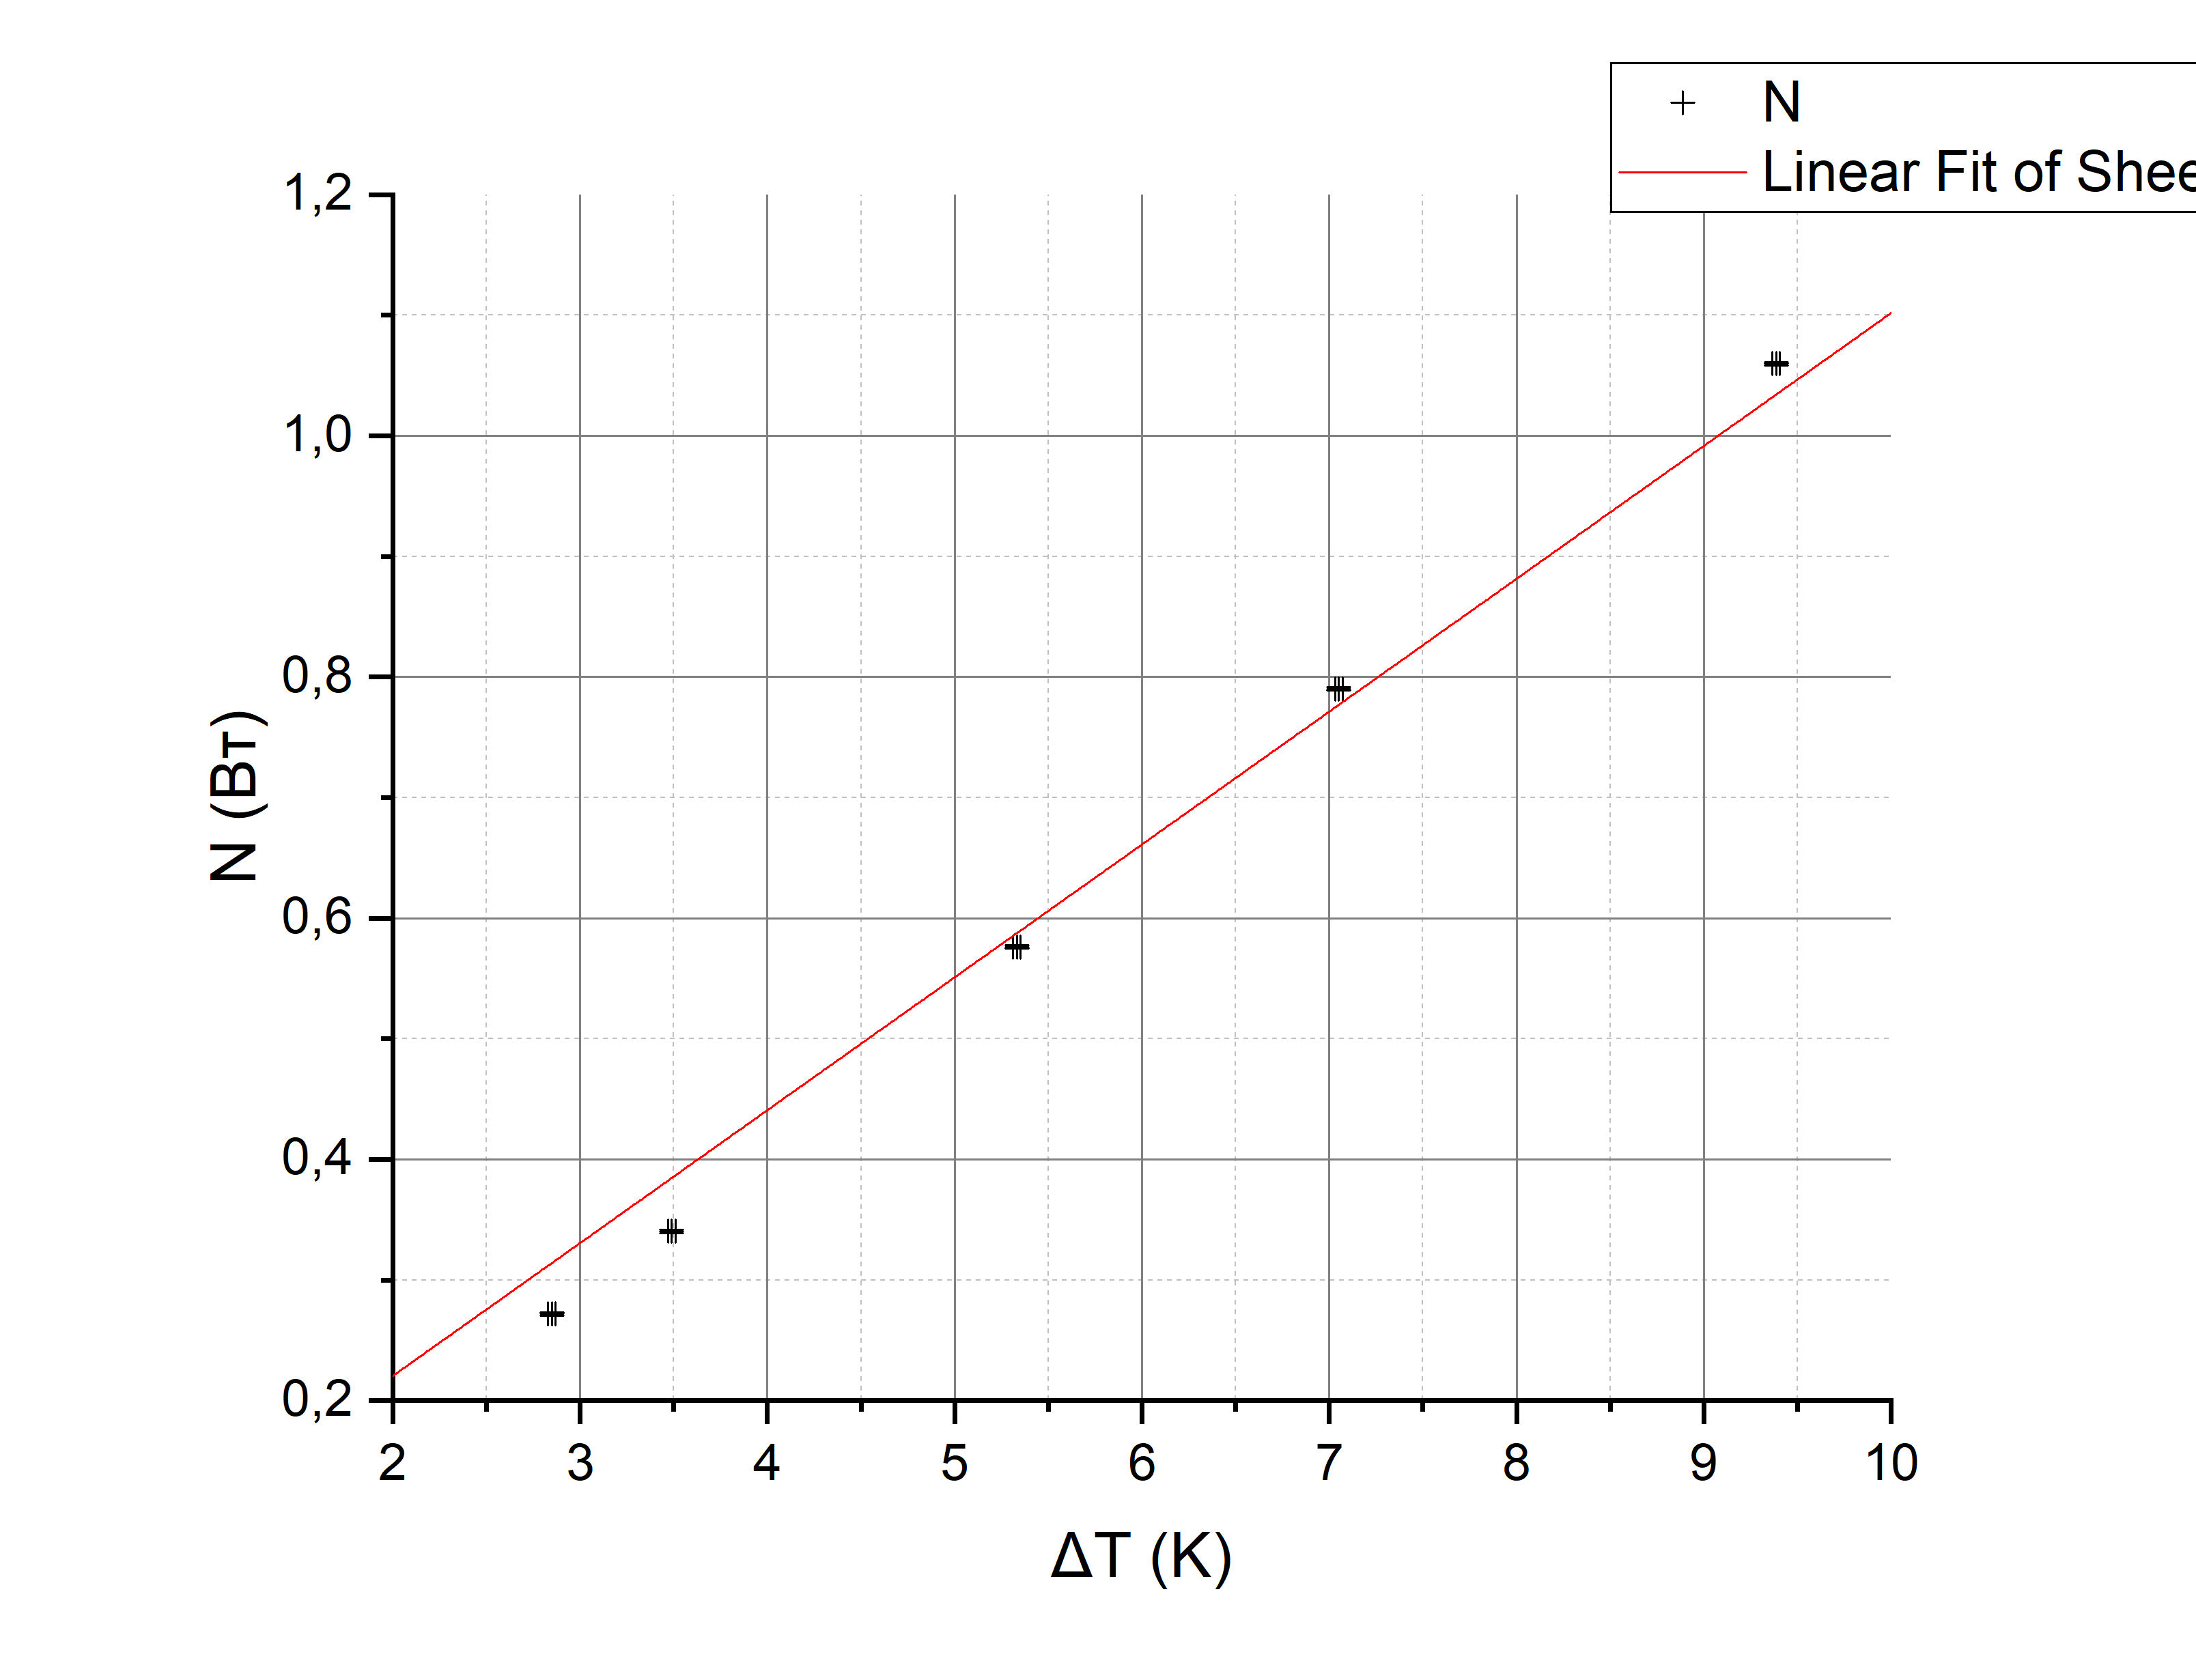
\includegraphics[width = \textwidth]{211_3.jpg}
    \textbf{График для $q_1$}
  \end{center} 
  \begin{center} 
    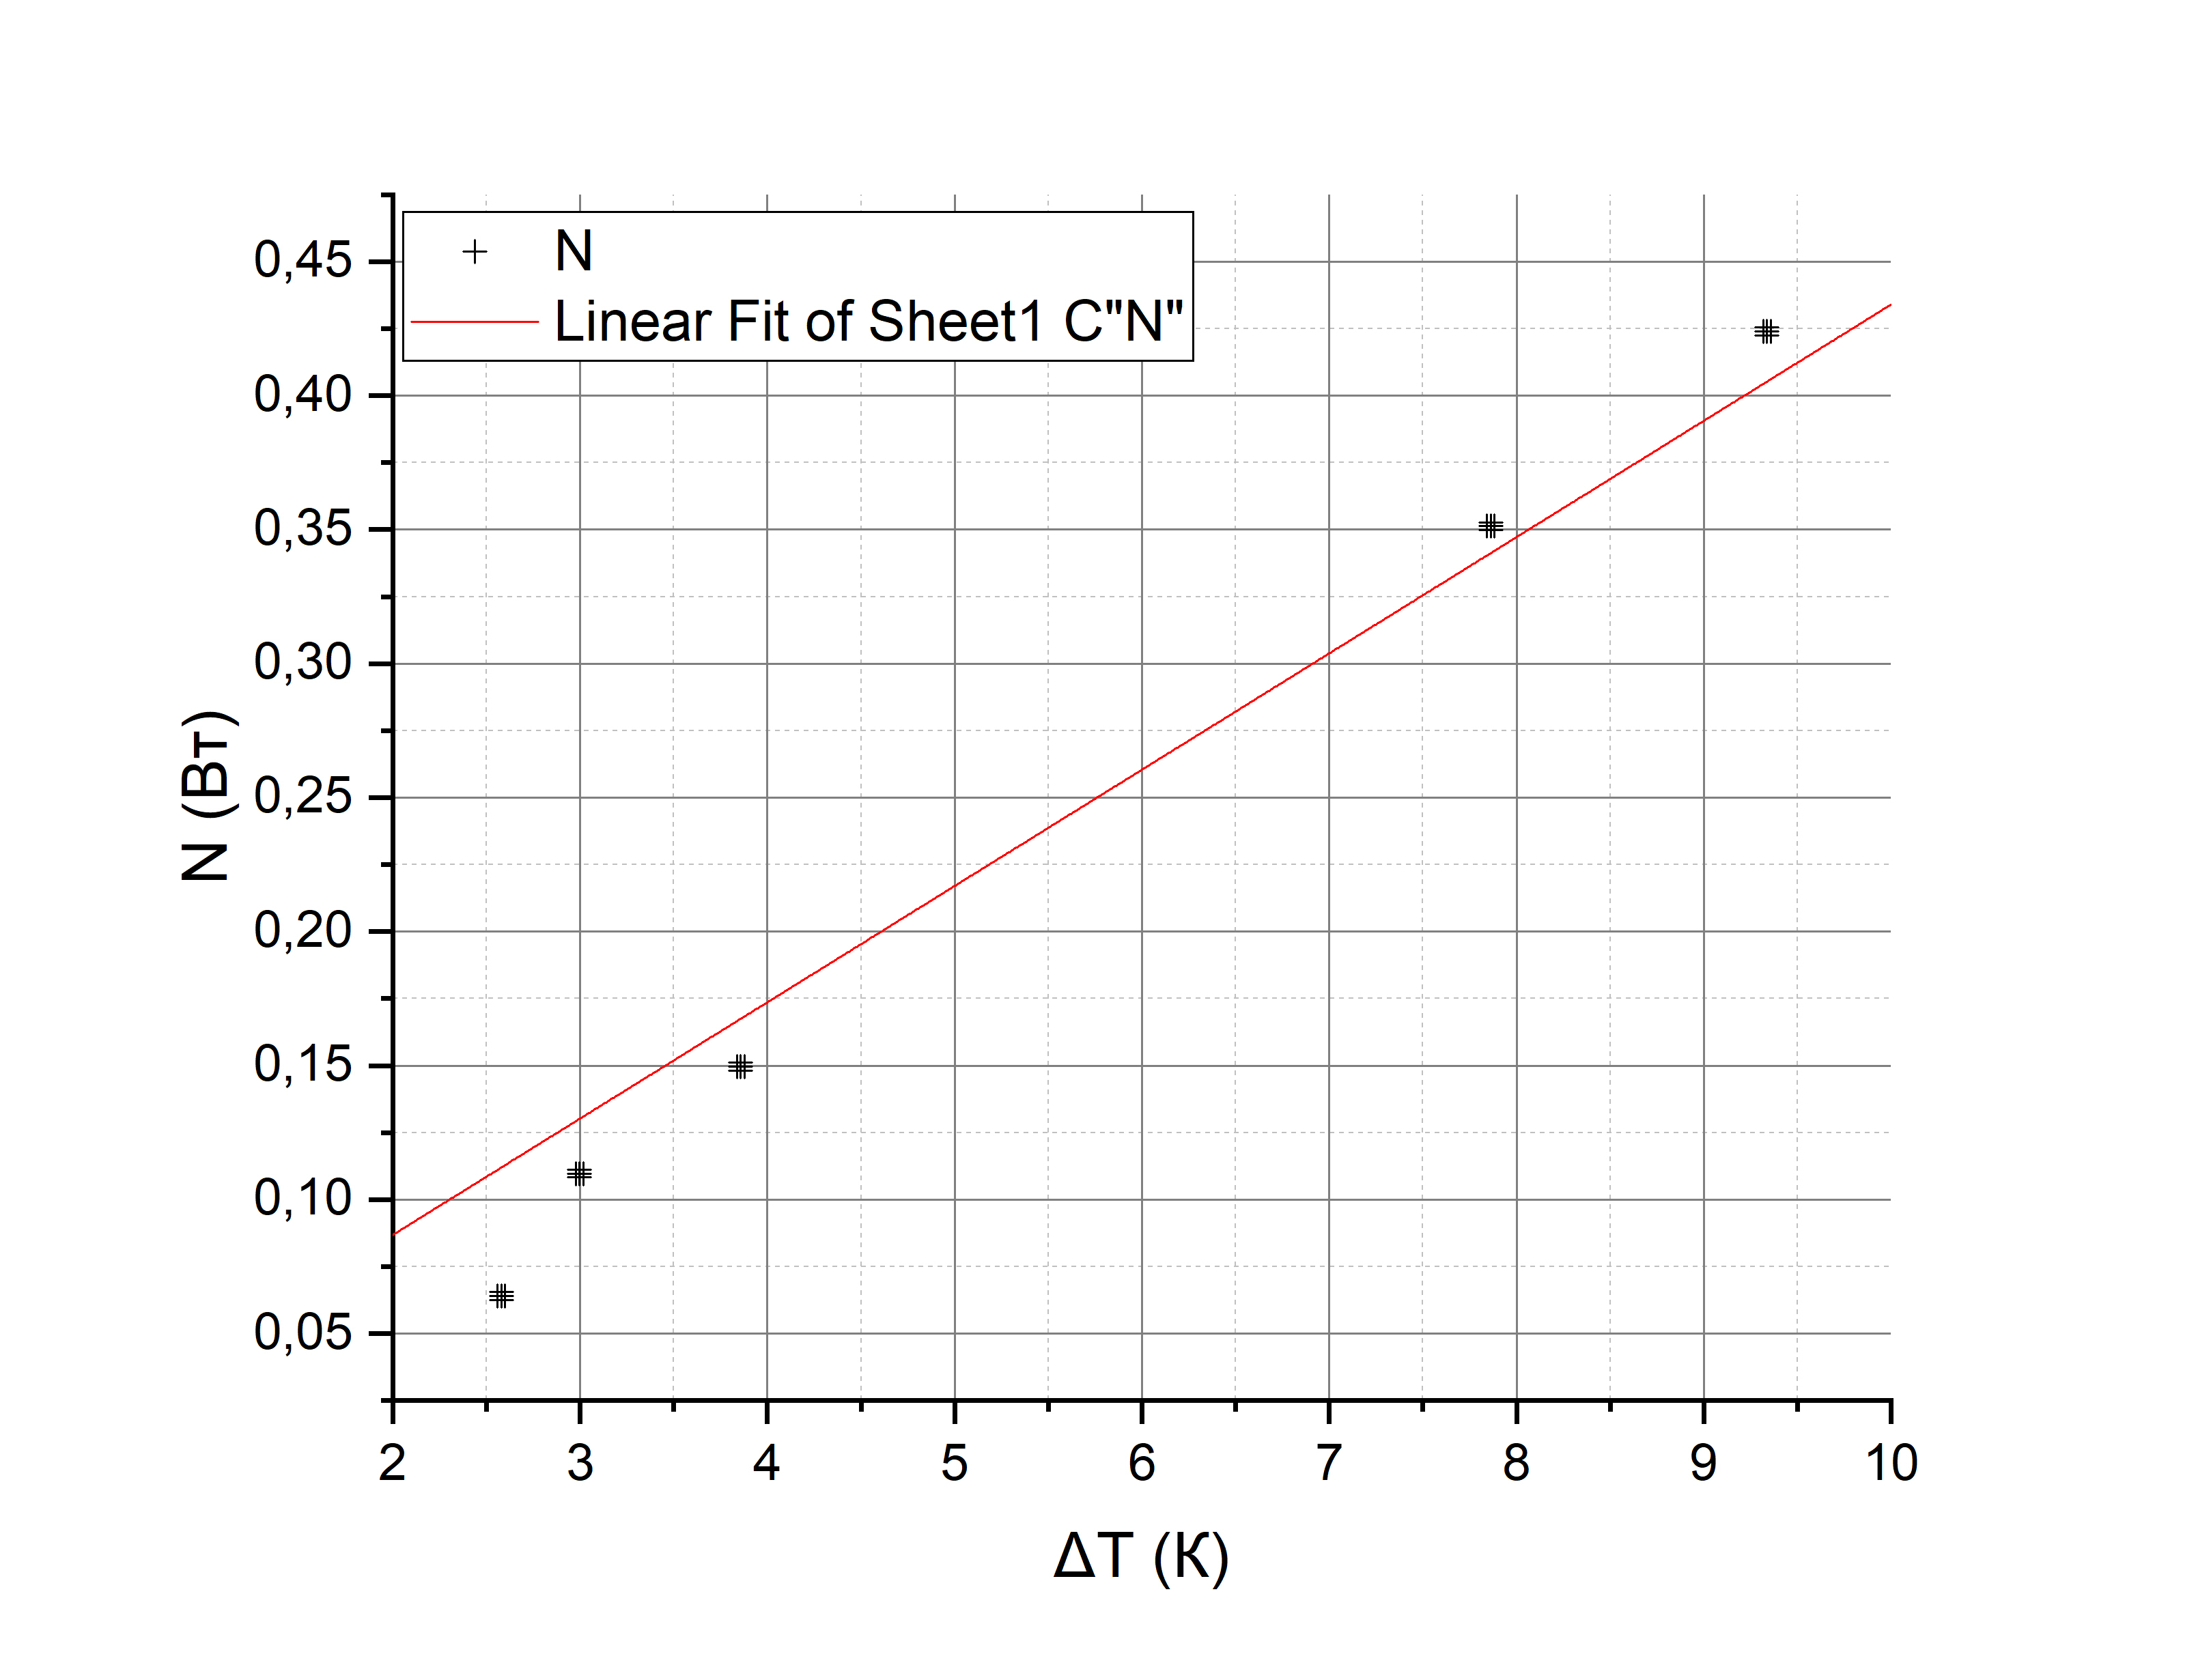
\includegraphics[width = \textwidth]{211_4.jpg}
    \textbf{График для $q_2$}
  \end{center}
   \begin{center}
    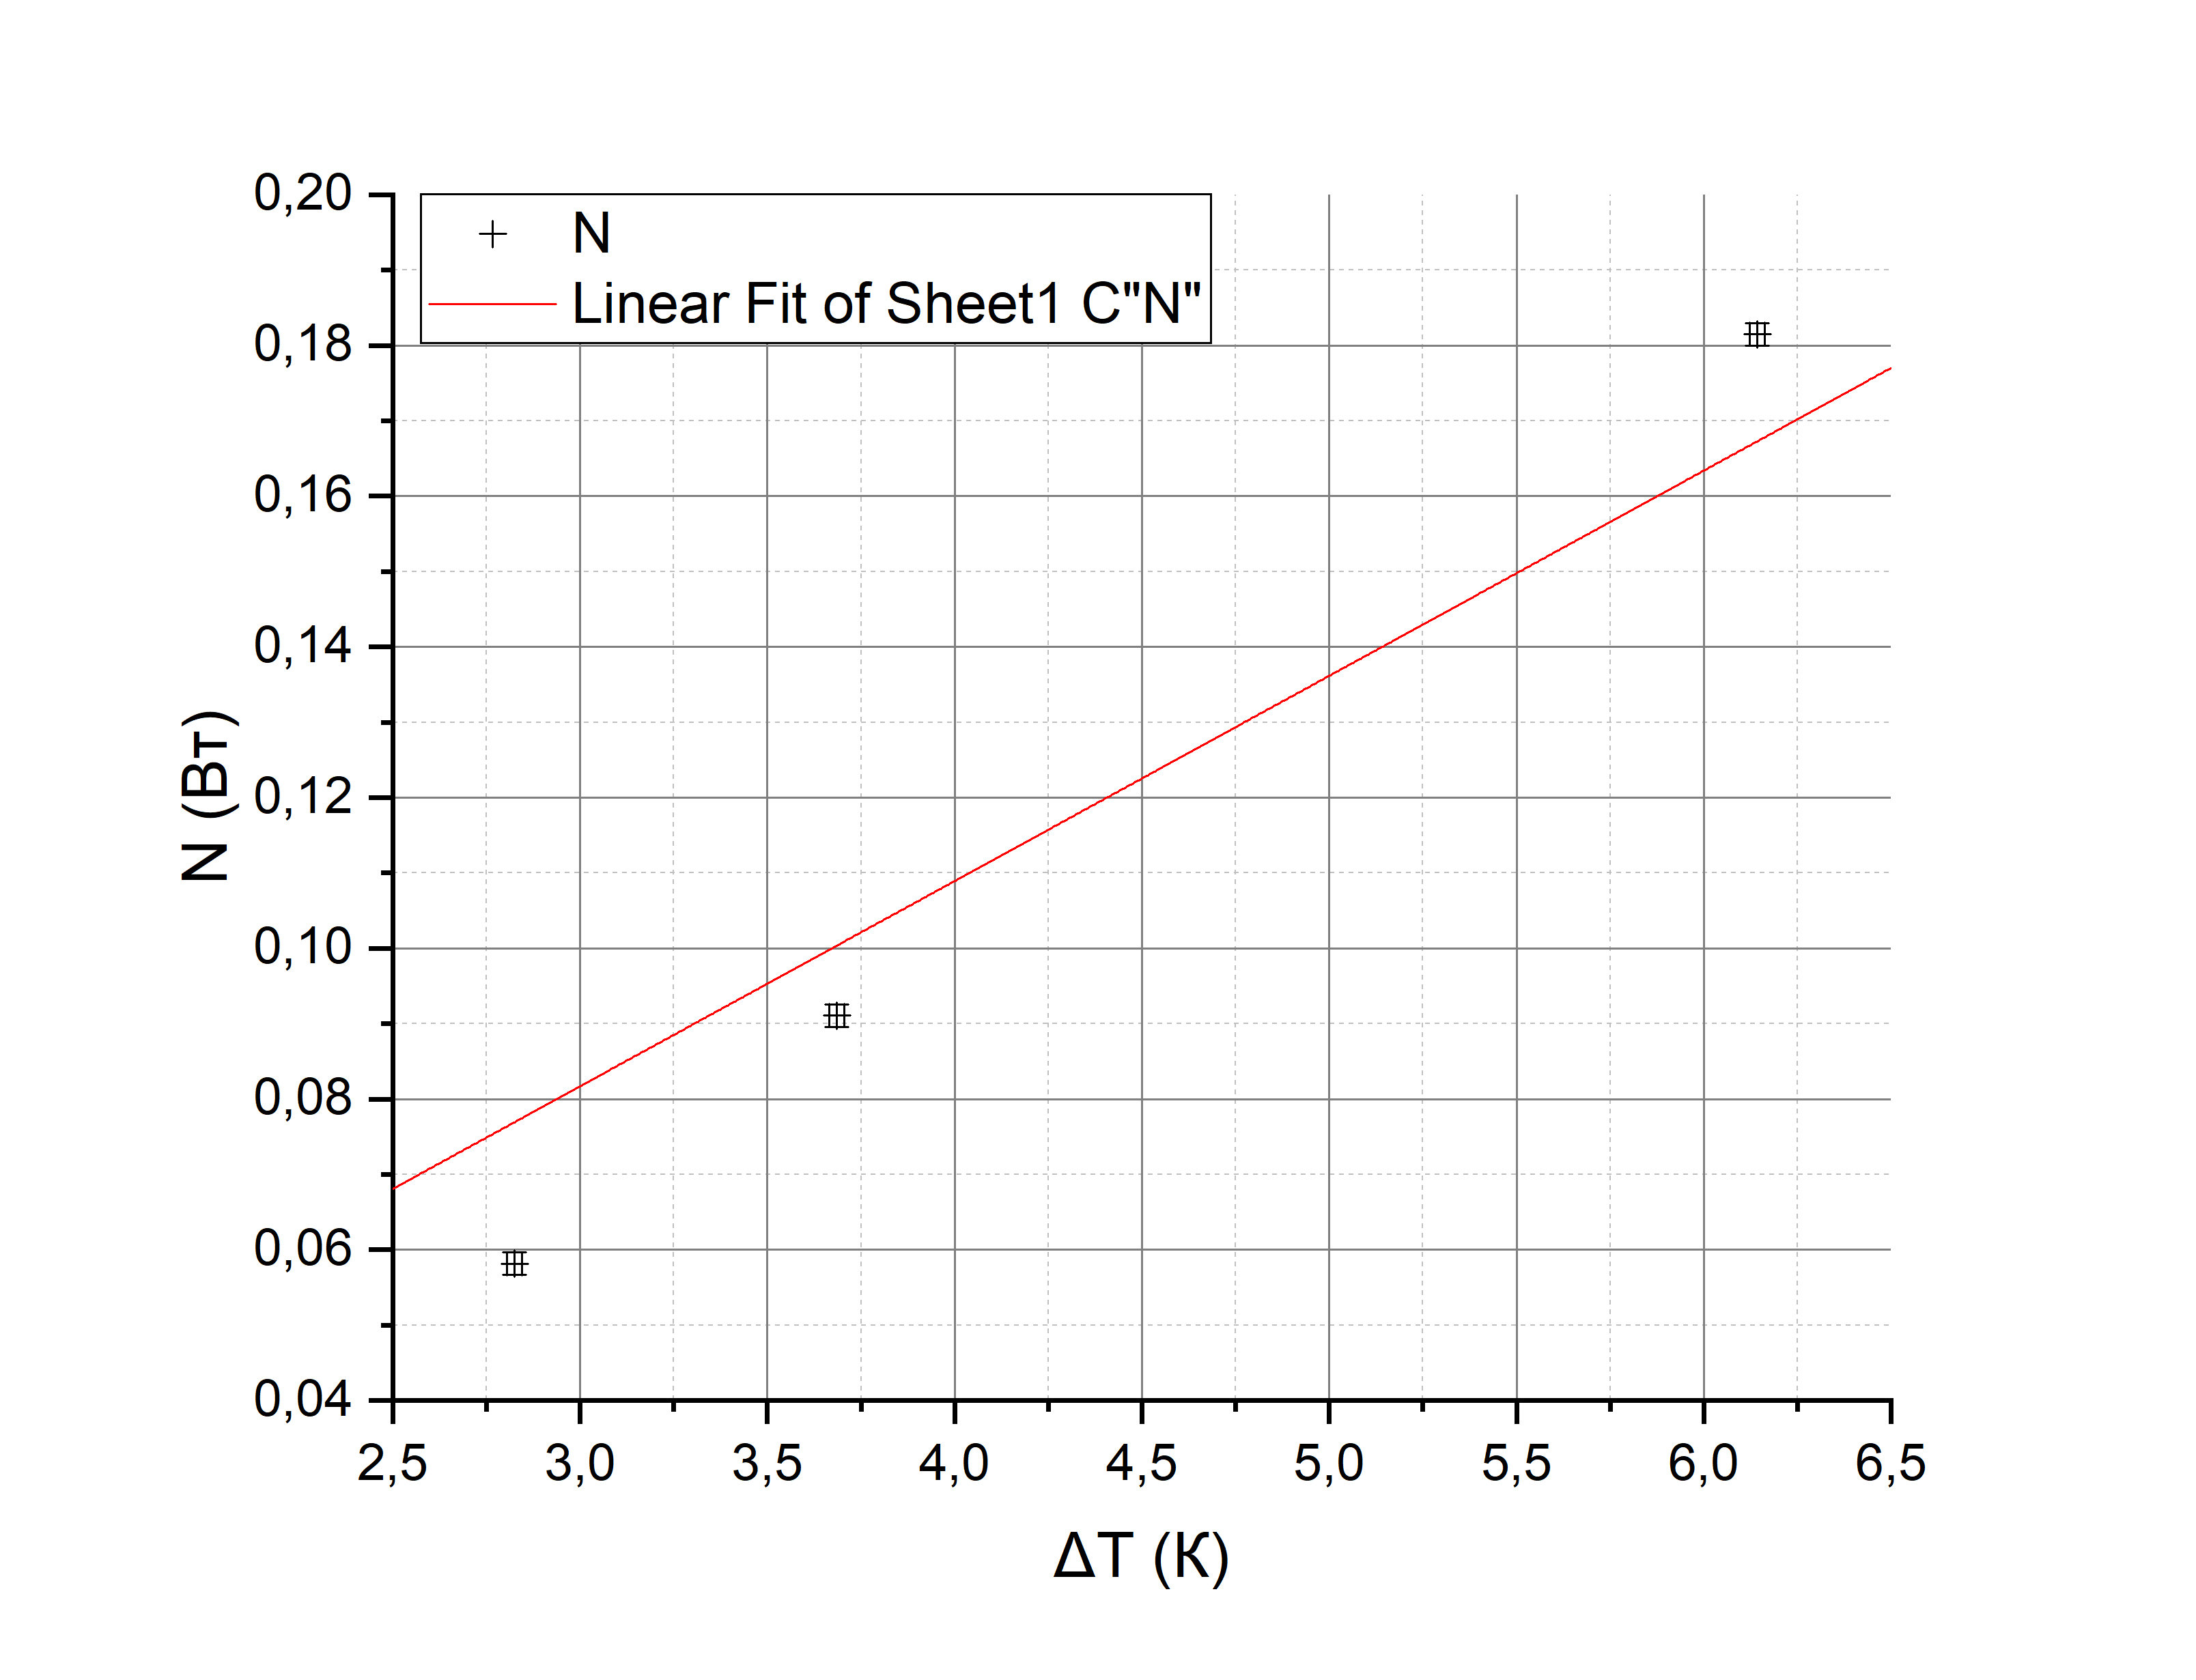
\includegraphics[width = \textwidth]{211_5.jpg}
      \textbf{График для $q_3$}
  \end{center}
\item [\textbf{10.}] Анализируем зависимость наклона $k$ от расхода $q$ и, пользуясь формулой (7), определяем $c_p \approx (3,81 \pm 0,3)R$ Дж/(моль $\cdot$ K), $N_{\text{пот}}/N \approx (0,007 \pm 0,0015)$.

\begin{tabular}{|c|c|c|c|}
\hline
$k$, Вт/K & $\sigma_k$, Вт/K & $q$, г/c & $\sigma_q$, г/c \\ \hline
0,11 & 0,006 & 0,095 & 0,002 \\ \hline
0,044 & 0,006 & 0,033 & 0,002 \\ \hline
0,028 & 0,006 & 0,019 & 0,002 \\ \hline
\end{tabular}
\begin{center}
    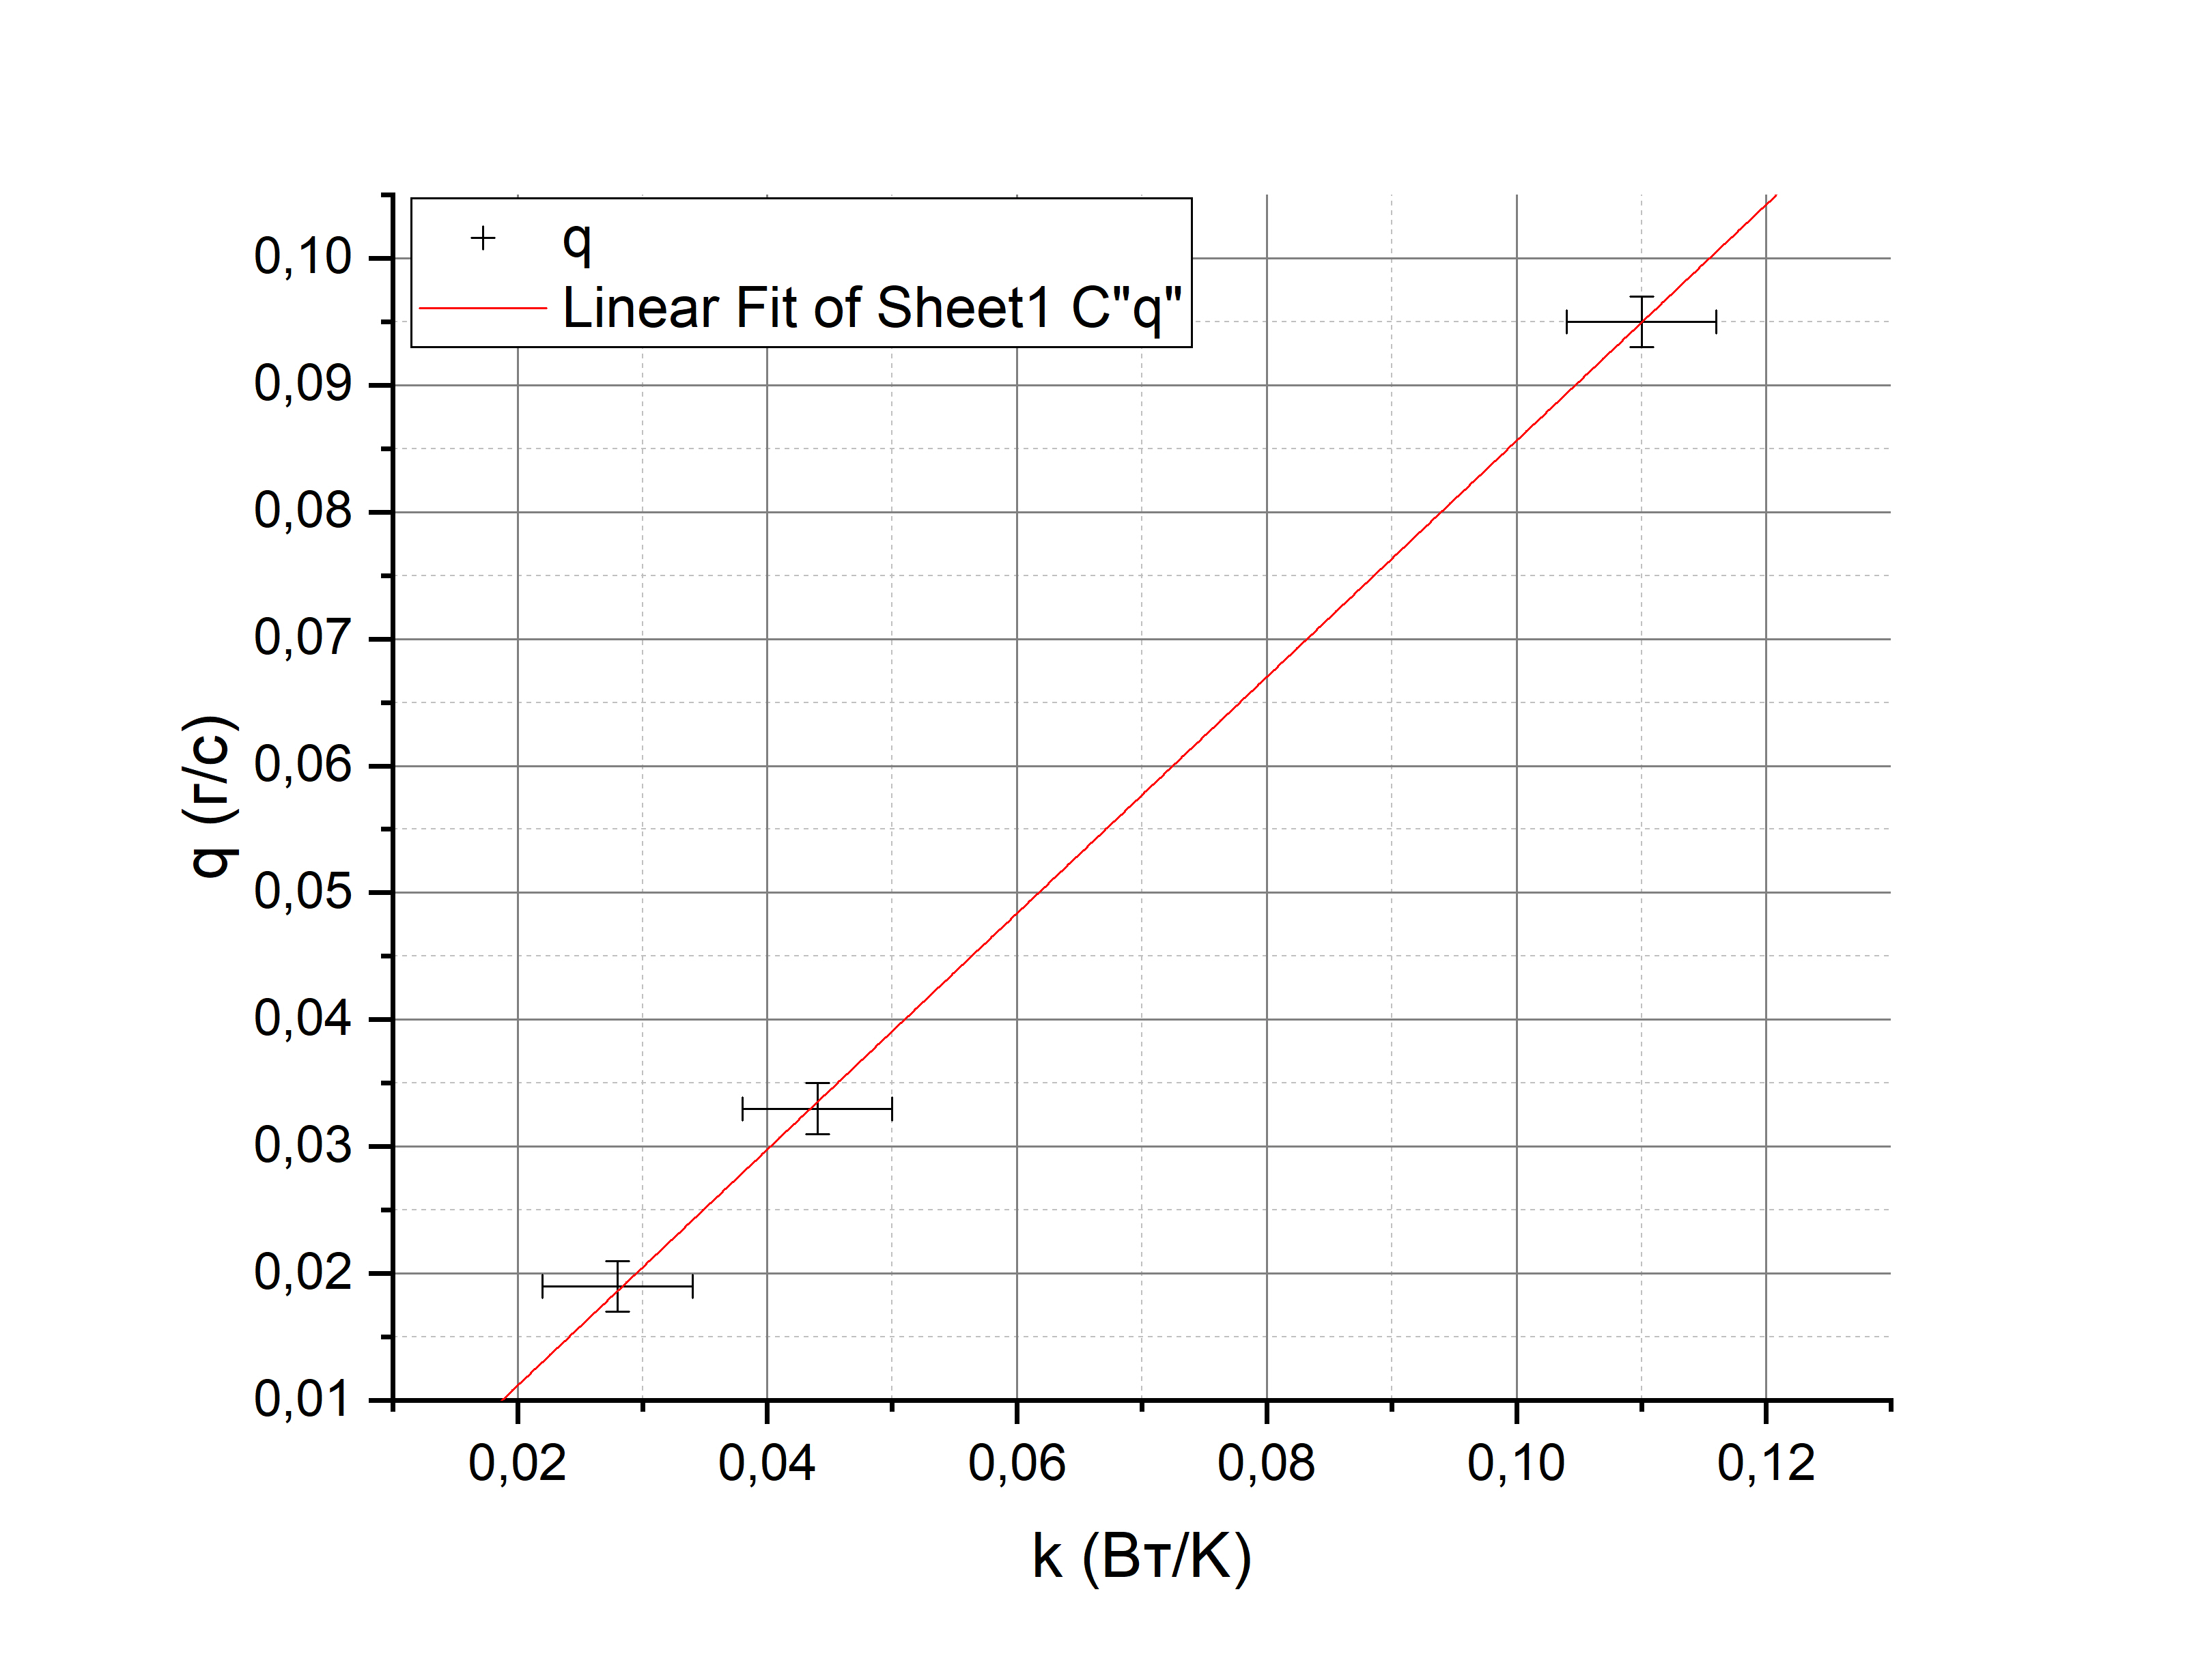
\includegraphics[width = \textwidth]{211_6.jpg}
      \textbf{График для $c_p$}
  \end{center}
\end{enumerate}
\end{document}